%%%%%%%%%%%%%%%%%%%%%%%%%%%%%%%%%%%%%%%%%%%%%%%%%%%%%%%%%%%%%%%%%%%%%%%%%%%%%%%%%%
\begin{frame}[fragile]\frametitle{}
\begin{center}
{\Large Implementation}
\end{center}
\end{frame}

%%%%%%%%%%%%%%%%%%%%%%%%%%%%%%%%%%%%%%%%%%%%%%%%%%%%%%%%%%%%%%%%%%%%%%%%%%%%%%%%%%
\begin{frame}[fragile]\frametitle{}
\begin{center}
{\Large Frameworks}

{\tiny (Ref: Vizuara AI Agents Bootcamp)}
\end{center}
\end{frame}


%%%%%%%%%%%%%%%%%%%%%%%%%%%%%%%%%%%%%%%%%%%%%%%%%%%%%%%%%%%
\begin{frame}[fragile]\frametitle{}

\begin{center}
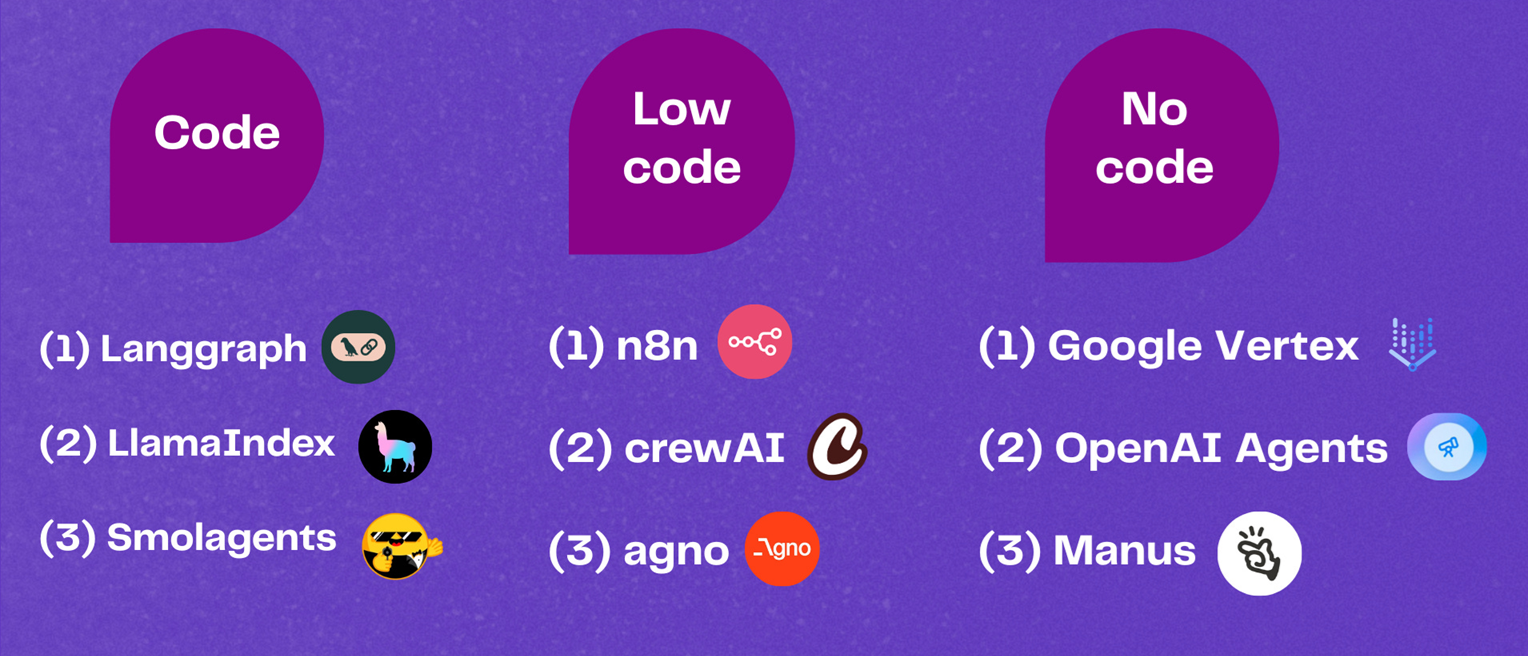
\includegraphics[width=\linewidth,keepaspectratio]{aiagents35}

{\tiny (Ref: Vizuara AI Agents Bootcamp)}
\end{center}	
  
\end{frame}

%%%%%%%%%%%%%%%%%%%%%%%%%%%%%%%%%%%%%%%%%%%%%%%%%%%%%%%%%%%
\begin{frame}[fragile]\frametitle{LangChain: The OG Agent Framework}
      \begin{itemize}
	  \item Open-source library connecting LLMs with data and APIs
	  \item Launched late 2022, fastest-growing GitHub project by mid-2023
	  \item Provides modular components: prompts, memory, tools, interfaces
	  \item Enables building chatbots to autonomous agents
	  \item General-purpose toolkit for LLM applications
	  \item Used by thousands of developers worldwide
	  \item Chain-based approach for sequential operations
	  \item Foundation for many other agent frameworks
	  \end{itemize}
\end{frame}

%%%%%%%%%%%%%%%%%%%%%%%%%%%%%%%%%%%%%%%%%%%%%%%%%%%%%%%%%%%
\begin{frame}[fragile]\frametitle{LangGraph: Graph-Based Agent Orchestration}
      \begin{itemize}
	  \item Newer framework from LangChain team with graph approach
	  \item Defines graphs of steps and decision points vs linear chains
	  \item Enables complex workflows with conditional branching
	  \item More low-level and controllable than LangChain agents
	  \item Charts exactly how AI navigates tasks like a map
	  \item Handles multiple possible sub-tasks efficiently
	  \item Ideal for complex decision flows and routing
	  \item Provides granular control over agent behavior
	  \end{itemize}
\end{frame}

%%%%%%%%%%%%%%%%%%%%%%%%%%%%%%%%%%%%%%%%%%%%%%%%%%%%%%%%%%%
\begin{frame}[fragile]\frametitle{LlamaIndex: LLMs + Your Data}
      \begin{itemize}
	  \item Formerly GPT Index, specializes in retrieval-augmented generation
	  \item Go-to framework for connecting LLMs with external datasets
	  \item Indexes knowledge bases for intelligent fact retrieval
	  \item Pre-built agents for question-answering scenarios
	  \item Integrates with databases, vector stores, and APIs
	  \item Enables agents to access specific data beyond base LLM knowledge
	  \item Powers document-based and enterprise knowledge systems
	  \item Essential for data-grounded AI applications
	  \end{itemize}
\end{frame}

%%%%%%%%%%%%%%%%%%%%%%%%%%%%%%%%%%%%%%%%%%%%%%%%%%%%%%%%%%%
\begin{frame}[fragile]\frametitle{SmolAgents: Minimalist Code-First Approach}
      \begin{itemize}
	  \item Hugging Face framework emphasizing simplicity and efficiency
	  \item Powerful agents in just a few lines of code
	  \item "Code-as-actions" philosophy: agents write Python directly
	  \item Up to 30\% fewer steps and API calls vs verbose instructions
	  \item Core logic only ~1000 lines of code
	  \item Lightweight and developer-friendly
	  \item Agents execute code for math, web scraping, etc.
	  \item Quick deployment without overhead
	  \end{itemize}
\end{frame}

%%%%%%%%%%%%%%%%%%%%%%%%%%%%%%%%%%%%%%%%%%%%%%%%%%%%%%%%%%%
\begin{frame}[fragile]\frametitle{Autogen: Multi-Agent Communication}
      \begin{itemize}
	  \item Microsoft framework for multi-agent conversations
	  \item Models applications as conversations between specialized agents
	  \item Supports group chats, hierarchical chats, human-in-the-loop
	  \item Agents can execute code in various environments
	  \item Enables AI pair-programming scenarios
	  \item Multiple agents critique and refine solutions collectively
	  \item Ideal for tasks requiring multiple perspectives
	  \item Pushes envelope on agent collaboration
	  \end{itemize}
\end{frame}

%%%%%%%%%%%%%%%%%%%%%%%%%%%%%%%%%%%%%%%%%%%%%%%%%%%%%%%%%%%
\begin{frame}[fragile]\frametitle{LangFlow: Visual LangChain Interface}
      \begin{itemize}
	  \item Web-based graphical UI for building LangChain flows
	  \item Drag-and-drop components instead of coding
	  \item Visualizes agent "thought" processes interactively
	  \item Lowers entry barrier for non-developers
	  \item Rapid prototyping and experimentation tool
	  \item Abstracts LangChain complexity for convenience
	  \item Configure prompts, models, memory through UI
	  \item Same capabilities as LangChain, visual interface
	  \end{itemize}
\end{frame}

%%%%%%%%%%%%%%%%%%%%%%%%%%%%%%%%%%%%%%%%%%%%%%%%%%%%%%%%%%%
\begin{frame}[fragile]\frametitle{CrewAI: Team-Based Agent Collaboration}
      \begin{itemize}
	  \item Framework inspired by human team collaboration
	  \item Sets up multiple agents with different roles in "crews"
	  \item High-level configuration over coding approach
	  \item Example: Researcher agent + Writer agent collaboration
	  \item Abstractions for tasks, planning, memory types
	  \item Developer-friendly with common patterns handled
	  \item Semi-finished assembly approach vs raw toolkits
	  \item Excellent for workflows breaking into sub-tasks
	  \end{itemize}
\end{frame}




%%%%%%%%%%%%%%%%%%%%%%%%%%%%%%%%%%%%%%%%%%%%%%%%%%%%%%%%%%%
\begin{frame}[fragile]\frametitle{n8n: Visual Workflow Automation with AI}
      \begin{itemize}
	  \item Open-source automation tool with LLM agent integration
	  \item Drag-and-drop workflow editor like visual Zapier
	  \item AI agent nodes operate within automated workflows
	  \item Maintains conversation context and calls tools
	  \item Visual orchestration mixing AI with enterprise tools
	  \item Example: Auto-analyze support tickets and recommend responses
	  \item Human review integration for quality control
	  \item Conductor for LLM agents in enterprise environments
	  \end{itemize}
\end{frame}

%%%%%%%%%%%%%%%%%%%%%%%%%%%%%%%%%%%%%%%%%%%%%%%%%%%%%%%%%%%
\begin{frame}[fragile]\frametitle{Manus: General-Purpose Autonomous Agent}
      \begin{itemize}
	  \item No-code platform claiming "AI employee" capabilities
	  \item Operates through chat interface with high-level goals
	  \item Plans and executes tasks autonomously over hours/days
	  \item Internal cognition engine with API calls, web browsing
	  \item Continuous operation without supervision
	  \item Internal feedback loop and memory for progress tracking
	  \item Actively uses tools: code execution, web queries, file operations
	  \item Beyond typical ChatGPT: keeps going until task completion
	  \end{itemize}
\end{frame}

%%%%%%%%%%%%%%%%%%%%%%%%%%%%%%%%%%%%%%%%%%%%%%%%%%%%%%%%%%%
\begin{frame}[fragile]\frametitle{Framework Recommendations by Category}
      \begin{itemize}
	  \item Code-level: LangGraph (graph orchestration), LangChain (general toolkit)
	  \item Code-level: LlamaIndex (data integration), SmolAgents (minimalist)
	  \item Low-code: CrewAI (team collaboration), LangFlow (visual workflows)
	  \item Low-code: n8n (enterprise automation), Agno (full-stack performance)
	  \item No-code: Manus (autonomous agents), OpenAI Deep Research
	  \item No-code: Gemini Deep Research for specialized tasks
	  \item Choose based on technical expertise and use case complexity
	  \item Consider team skills, maintenance requirements, and scalability needs
	  \end{itemize}
\end{frame}


%%%%%%%%%%%%%%%%%%%%%%%%%%%%%%%%%%%%%%%%%%%%%%%%%%%%%%%%%%%
\begin{frame}[fragile]\frametitle{Langfuse: Tracing and Evaluation}
% \begin{columns}
    % \begin{column}[T]{0.6\linewidth}
      \begin{itemize}
		\item Complete Execution Tracing: Records every agent step and tool usage
		\item Timeline Visualization: Shows sequence of operations and model calls
		\item Agent Message Logging: Captures prompts and responses between agents
		\item Tool Usage Tracking: Monitors exact queries and results from each tool
		\item Performance Metrics: Measures latency, token usage, and quality scores
		\item Production Monitoring: Essential for reliable agent deployment
	  \end{itemize}
    % \end{column}
    % \begin{column}[T]{0.4\linewidth}
		\begin{center}
		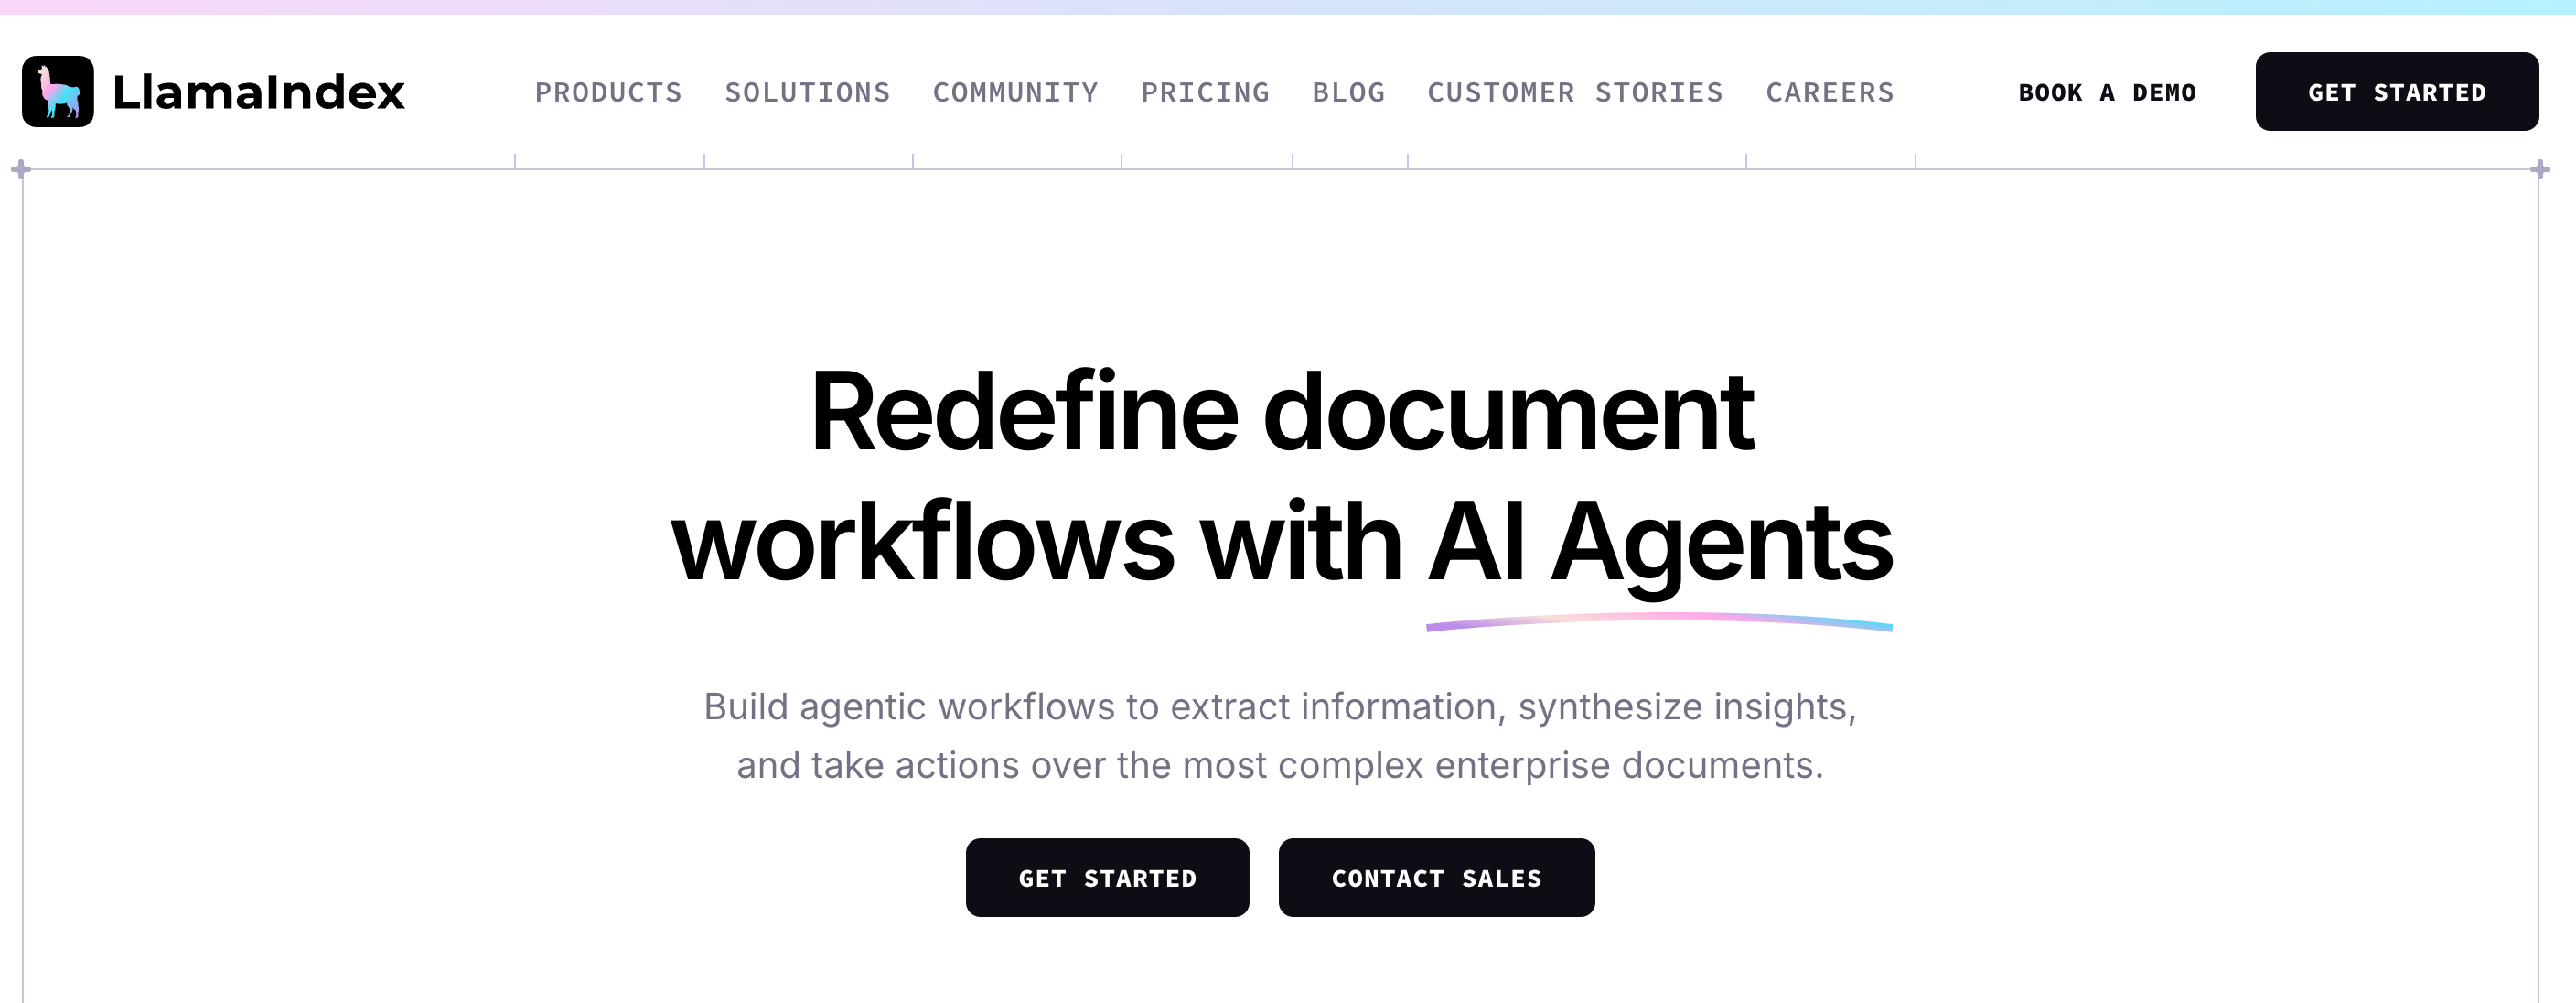
\includegraphics[width=0.8\linewidth,keepaspectratio]{aiagents58}
		
		{\tiny (Ref: Vizuara AI Agents Bootcamp)}
		\end{center}	
    % \end{column}
  % \end{columns}
\end{frame}


%%%%%%%%%%%%%%%%%%%%%%%%%%%%%%%%%%%%%%%%%%%%%%%%%%%%%%%%%%%
\begin{frame}[fragile]\frametitle{Arize Phoenix: Production Observability}
% \begin{columns}
    % \begin{column}[T]{0.6\linewidth}
      \begin{itemize}
		\item Open-Source Platform: LLM observability and evaluation for production systems
		\item Trace Visualization: Tree view of agent actions and reasoning steps
		\item Performance Metrics: Latency, token count, and quality score tracking
		\item Error Detection: Identifies problematic spans and execution failures
		\item Callback Integration: Easy setup with LlamaIndex callback handlers
		\item Production Monitoring: Essential for trust and reliability in deployed agents
	  \end{itemize}
    % \end{column}
    % \begin{column}[T]{0.4\linewidth}
		\begin{center}
		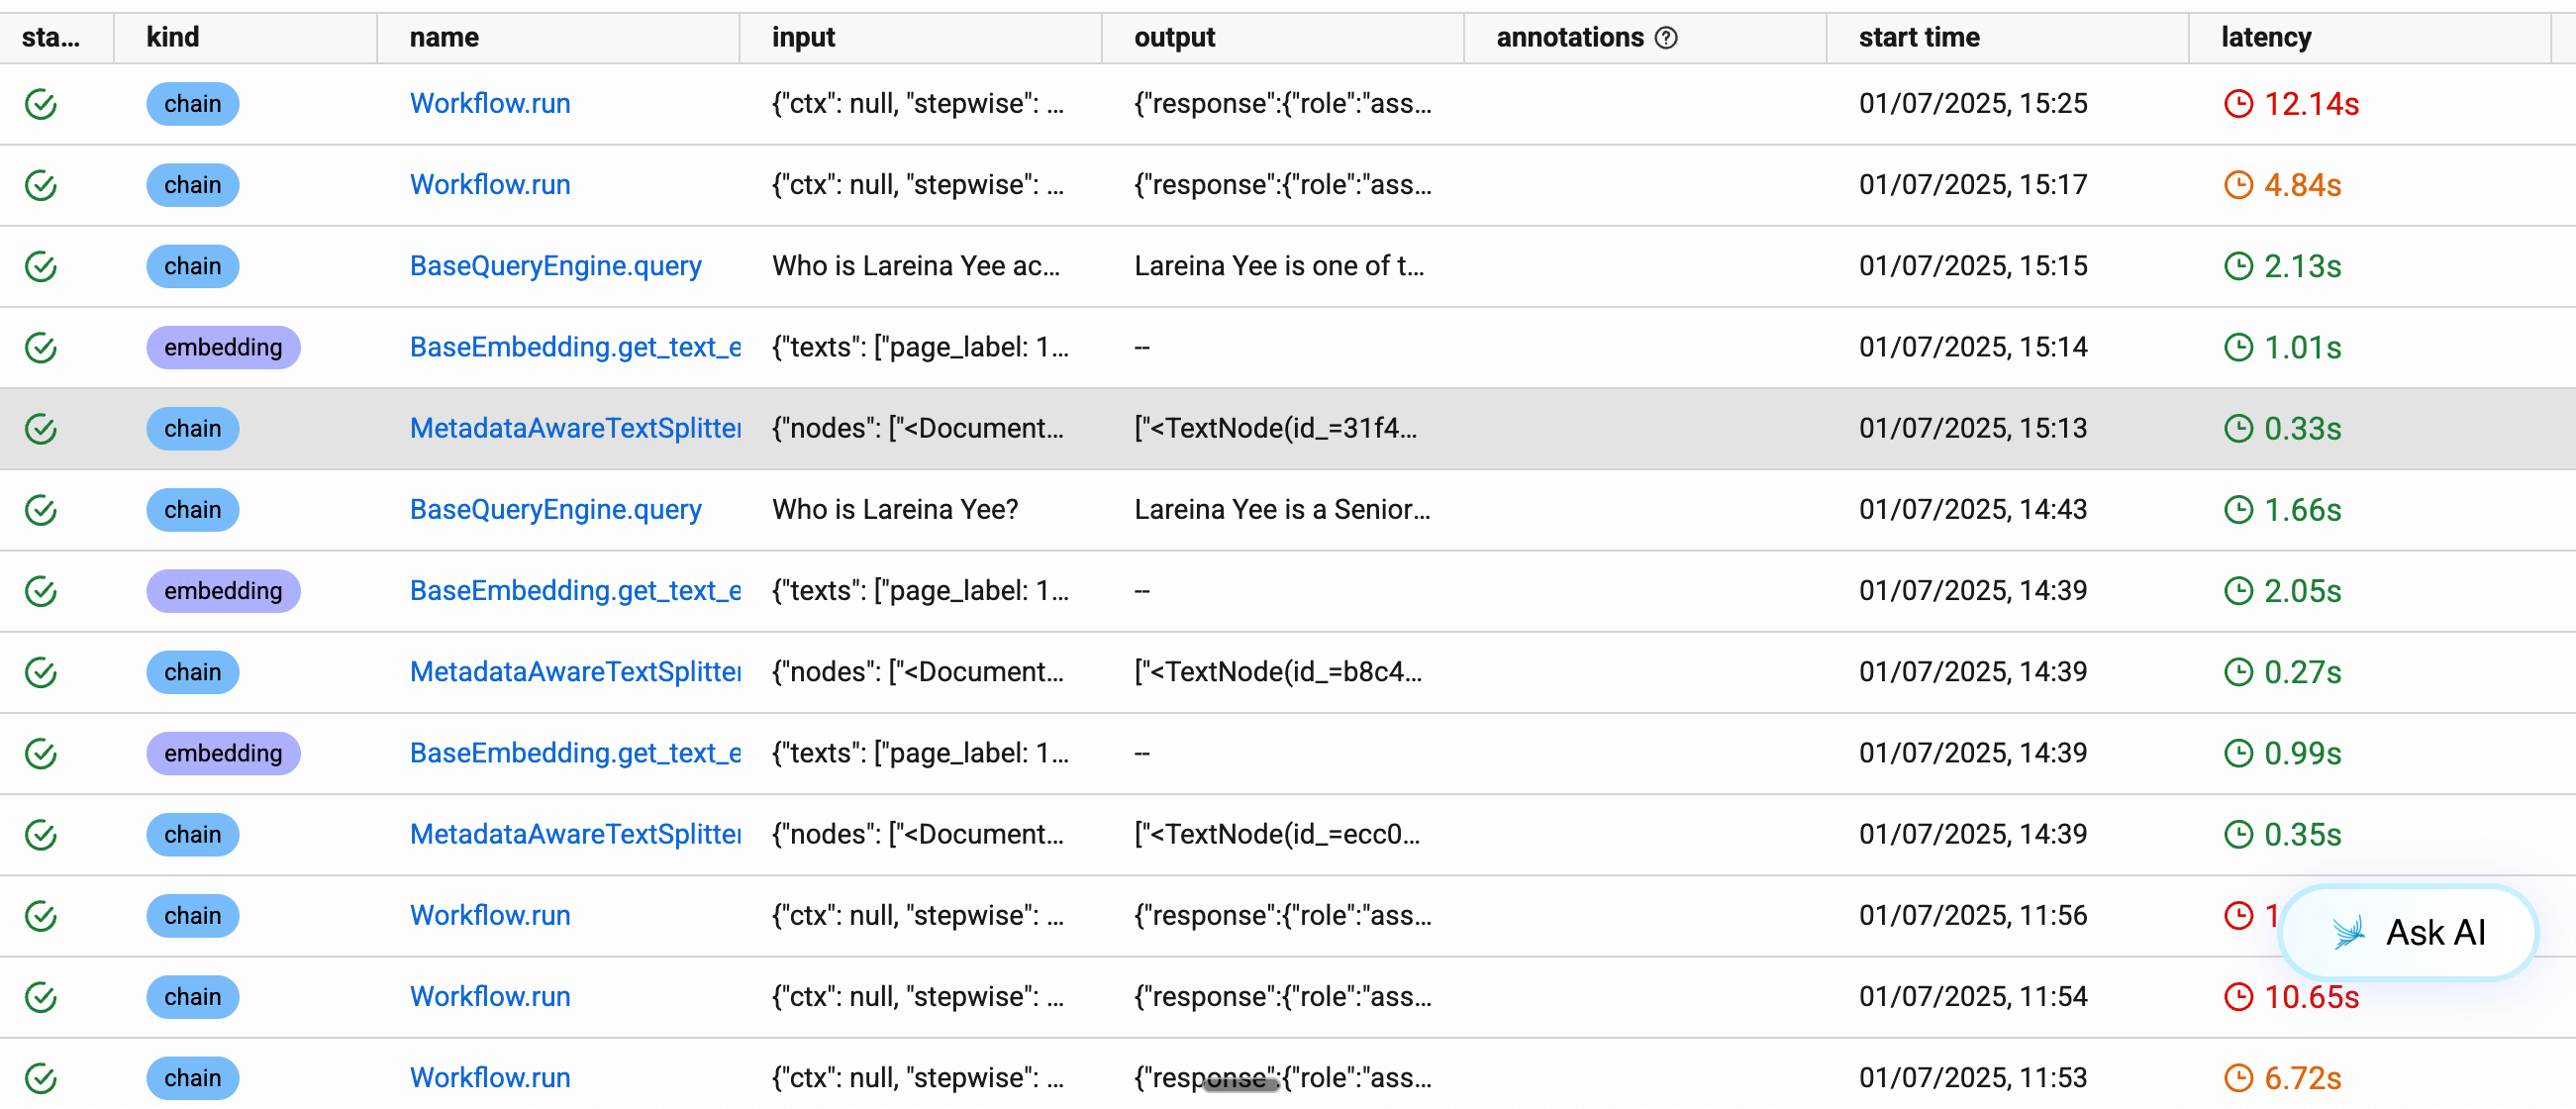
\includegraphics[width=0.6\linewidth,keepaspectratio]{aiagents63}
		\end{center}	
    % \end{column}
  % \end{columns}
\end{frame}

%%%%%%%%%%%%%%%%%%%%%%%%%%%%%%%%%%%%%%%%%%%%%%%%%%%%%%%%%%%
\begin{frame}[fragile]\frametitle{Future Directions and Extensions}
% \begin{columns}
    % \begin{column}[T]{0.6\linewidth}
      \begin{itemize}
		\item Multi-Agent Orchestration: Multiple specialized agents working together
		\item Real-Time Data Integration: Live APIs and streaming data sources
		\item Advanced Tool Ecosystem: Expanding LlamaHub with custom tools
		\item Workflow Automation: Complex business process automation with agent chains
		\item Quality Assurance: Automated evaluation and continuous improvement loops
		\item Production Scaling: Enterprise deployment with monitoring and governance
	  \end{itemize}
    % \end{column}
    % \begin{column}[T]{0.4\linewidth}
		% \begin{center}
		% \includegraphics[width=0.8\linewidth,keepaspectratio]{future_directions}
		% \end{center}	
    % \end{column}
  % \end{columns}
\end{frame}

%%%%%%%%%%%%%%%%%%%%%%%%%%%%%%%%%%%%%%%%%%%%%%%%%%%%%%%%%%%
\begin{frame}[fragile]\frametitle{}

\begin{center}
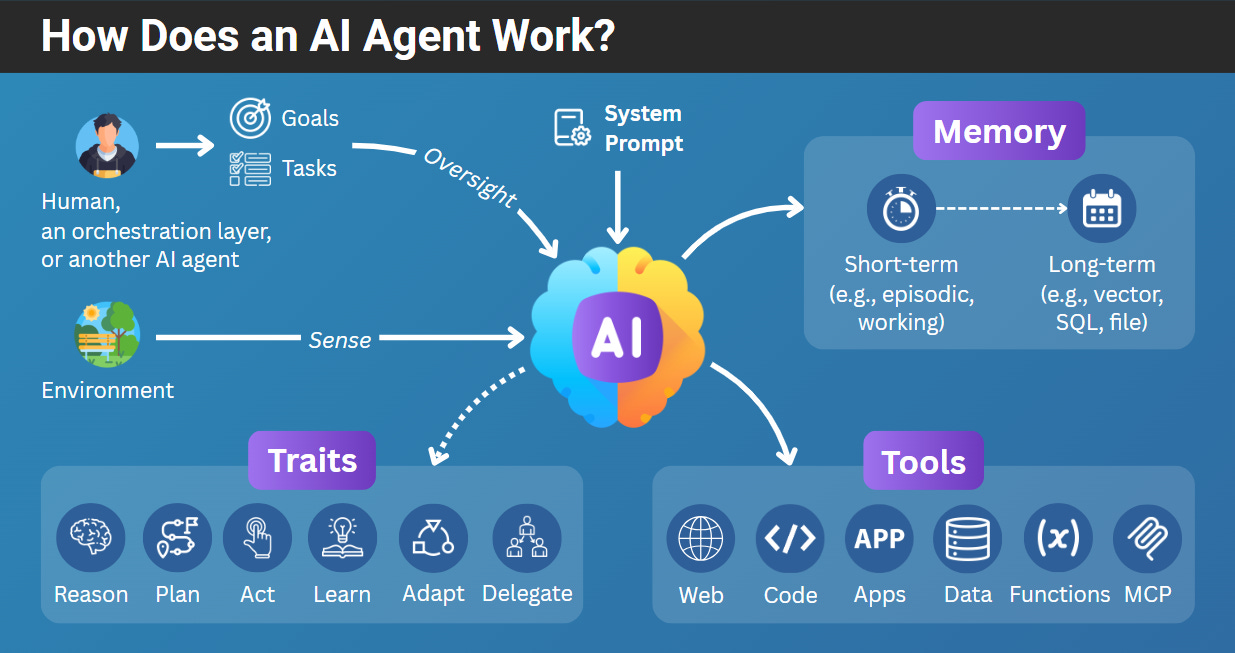
\includegraphics[width=\linewidth,keepaspectratio]{aiagents5}

{\tiny (Ref: The Ultimate Guide to AI Agents for PMs - Pawl Huryn)}
\end{center}	
  
\end{frame}

%%%%%%%%%%%%%%%%%%%%%%%%%%%%%%%%%%%%%%%%%%%%%%%%%%%%%%%%%%%
\begin{frame}[fragile]\frametitle{Build Your First AI Agent}
      \begin{itemize}
        \item Takes just 30-60 minutes to get started
        \item Follow a clear step-by-step process
        \item Focus on functionality, not theory
      \end{itemize}
\end{frame}

%%%%%%%%%%%%%%%%%%%%%%%%%%%%%%%%%%%%%%%%%%%%%%%%%%%%%%%%%%%%%%%%%%%%%%%%%%%%%%%%%%
\begin{frame}[fragile]\frametitle{How to Build an AI Agent?}

	\begin{center}
	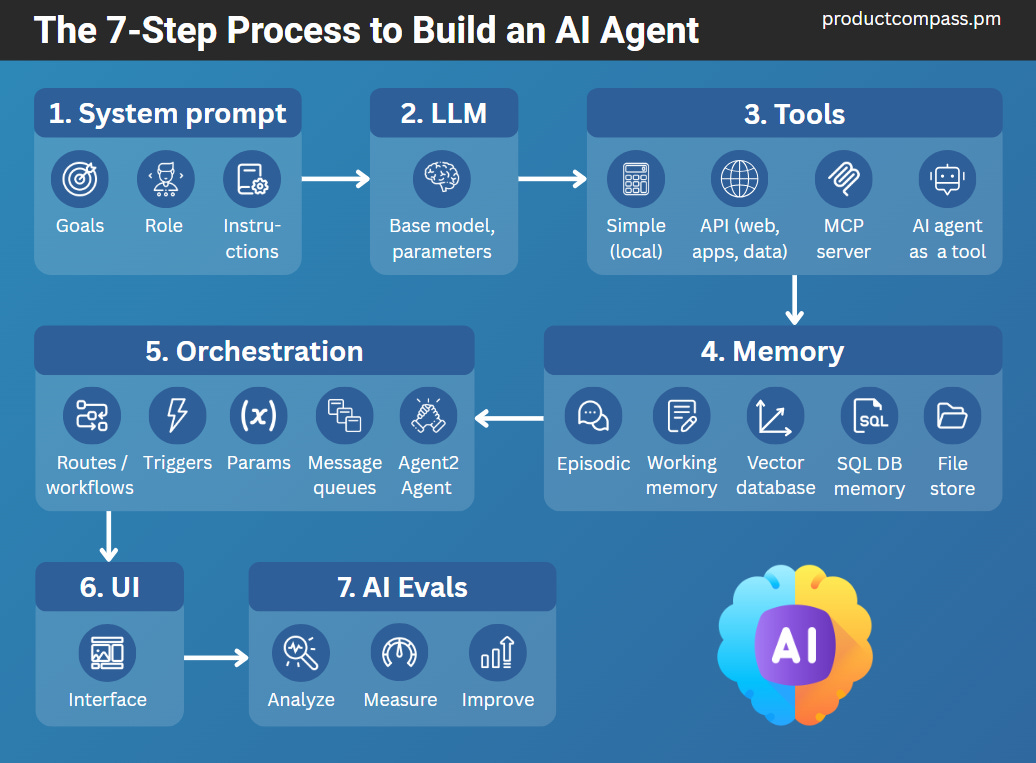
\includegraphics[width=0.8\linewidth,keepaspectratio]{aiagents7}
	\end{center}
	
	{\tiny (Ref: The Ultimate Guide to AI Agents for PMs - Pawl Huryn)}
\end{frame}


%%%%%%%%%%%%%%%%%%%%%%%%%%%%%%%%%%%%%%%%%%%%%%%%%%%%%%%%%%%
\begin{frame}[fragile]\frametitle{Step 1: Define a System Prompt}
      \begin{itemize}
        \item Set goals, logic, and expectations
        \item Use structured prompting principles
        \item Refer to expert guides for inspiration
      \end{itemize}
\end{frame}

%%%%%%%%%%%%%%%%%%%%%%%%%%%%%%%%%%%%%%%%%%%%%%%%%%%%%%%%%%%
\begin{frame}[fragile]\frametitle{Step 2: Select an LLM}
      \begin{itemize}
        \item Choose a reasoning-capable model (e.g., o1-mini)
        \item Frameworks like n8n may handle iterations
        \item Pick based on your use case complexity
      \end{itemize}
\end{frame}

%%%%%%%%%%%%%%%%%%%%%%%%%%%%%%%%%%%%%%%%%%%%%%%%%%%%%%%%%%%
\begin{frame}[fragile]\frametitle{Step 3: Connect Tools}
      \begin{itemize}
        \item Add tools based on agent goals
        \item Use calculators, functions, data sources
        \item Optional: MCP servers for integration
      \end{itemize}
\end{frame}

%%%%%%%%%%%%%%%%%%%%%%%%%%%%%%%%%%%%%%%%%%%%%%%%%%%%%%%%%%%
\begin{frame}[fragile]\frametitle{Step 4: Connect Memory}
      \begin{itemize}
        \item Enable short-term memory for local state
        \item Use long-term memory: vector, SQL, graph
        \item Essential for tracking progress and context
      \end{itemize}
\end{frame}

%%%%%%%%%%%%%%%%%%%%%%%%%%%%%%%%%%%%%%%%%%%%%%%%%%%%%%%%%%%
\begin{frame}[fragile]\frametitle{Step 5: Orchestrate the Logic}
      \begin{itemize}
        \item Map core logic not tied to a single agent
        \item Enable agent-to-agent communication
        \item Static or dynamic flows via orchestration
      \end{itemize}
\end{frame}

%%%%%%%%%%%%%%%%%%%%%%%%%%%%%%%%%%%%%%%%%%%%%%%%%%%%%%%%%%%
\begin{frame}[fragile]\frametitle{Step 6: Add User Interface}
      \begin{itemize}
        \item Use no-code tools like Lovable or Bolt
        \item Easily create interfaces without coding
        \item Great for user-facing agents and SaaS apps
      \end{itemize}
\end{frame}

%%%%%%%%%%%%%%%%%%%%%%%%%%%%%%%%%%%%%%%%%%%%%%%%%%%%%%%%%%%
\begin{frame}[fragile]\frametitle{Step 7: Evaluate the Agent}
      \begin{itemize}
        \item Skip fixed metrics-do error analysis
        \item Let performance metrics emerge naturally
        \item For RAG: evaluate retrieval and generation separately
      \end{itemize}
\end{frame}

%%%%%%%%%%%%%%%%%%%%%%%%%%%%%%%%%%%%%%%%%%%%%%%%%%%%%%%%%%%
\begin{frame}[fragile]\frametitle{Bottom Line: Just Start}
      \begin{itemize}
        \item Follow practical guides-many require no coding
        \item Use frameworks like n8n and tools like MCP
        \item Stop theorizing-start shipping real systems
      \end{itemize}
\end{frame}


%%%%%%%%%%%%%%%%%%%%%%%%%%%%%%%%%%%%%%%%%%%%%%%%%%%%%%%%%%%%%%%%%%%%%%%%%%%%%%%%%%
\begin{frame}[fragile]\frametitle{}
\begin{center}
{\Large Practical Tips}
\end{center}
\end{frame}

%%%%%%%%%%%%%%%%%%%%%%%%%%%%%%%%%%%%%%%%%%%%%%%%%%%%%%%%%%%
\begin{frame}[fragile]\frametitle{RAG vs. Fine-Tuning: Business Impact}
    \begin{itemize}
        \item Business-critical systems require the right LLM strategy.
        \item Fine-tuning feels powerful, but often adds avoidable complexity.
        \item Start by exploring simpler and more flexible approaches first.
    \end{itemize}
\end{frame}

%%%%%%%%%%%%%%%%%%%%%%%%%%%%%%%%%%%%%%%%%%%%%%%%%%%%%%%%%%%
\begin{frame}[fragile]\frametitle{RAG vs SFT}
	
	\begin{center}
	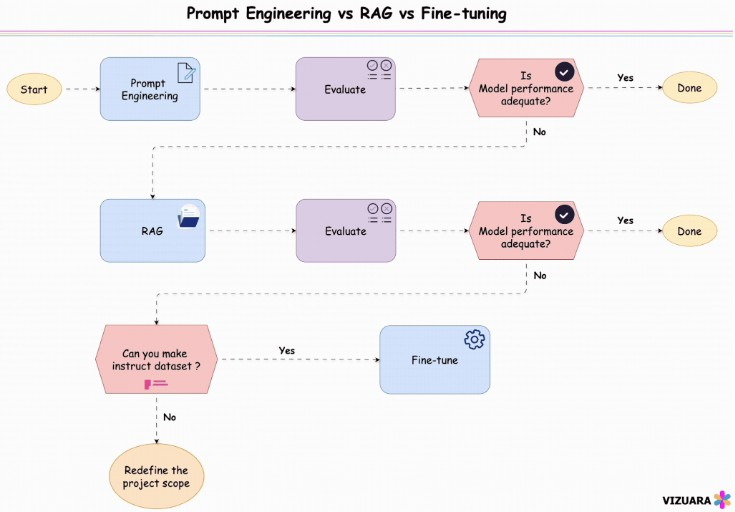
\includegraphics[width=0.8\linewidth,keepaspectratio]{vizuara1}
	\end{center}
	
{\tiny (Ref: LinkedIn post by Raj Dandekar)}

\end{frame}


%%%%%%%%%%%%%%%%%%%%%%%%%%%%%%%%%%%%%%%%%%%%%%%%%%%%%%%%%%%
\begin{frame}[fragile]\frametitle{Pre-Fine-Tuning Checklist}
    \begin{itemize}
        \item Can prompt engineering alone solve the task?
        \item Could Retrieval-Augmented Generation (RAG) help more?
        \item Is there a clear and testable system already in place?
    \end{itemize}
\end{frame}

%%%%%%%%%%%%%%%%%%%%%%%%%%%%%%%%%%%%%%%%%%%%%%%%%%%%%%%%%%%
\begin{frame}[fragile]\frametitle{Why RAG Outperformed Fine-Tuning}
    \begin{itemize}
        \item \textbf{Higher Accuracy}: Grounded answers from relevant context.
        \item \textbf{Fewer Hallucinations}: More reliable than fine-tuned outputs.
        \item \textbf{Dynamic Updates}: Easily update data without retraining models.
    \end{itemize}
\end{frame}

%%%%%%%%%%%%%%%%%%%%%%%%%%%%%%%%%%%%%%%%%%%%%%%%%%%%%%%%%%%
\begin{frame}[fragile]\frametitle{When to Use Fine-Tuning}
    \begin{itemize}
        \item RAG can't solve context window limitations.
        \item Domain-specific tone or behavior is required.
        \item The system is mature enough to absorb added complexity.
    \end{itemize}
\end{frame}

%%%%%%%%%%%%%%%%%%%%%%%%%%%%%%%%%%%%%%%%%%%%%%%%%%%%%%%%%%%
\begin{frame}[fragile]\frametitle{Strategy Summary}
    \begin{itemize}
        \item Prompt engineering solves 30--50\% of tasks.
        \item RAG adds power for another 30--40\%.
        \item Fine-tuning is best for the final 10\% of hard problems.
        \item Always choose the simplest effective approach first.
    \end{itemize}
\end{frame}

%%%%%%%%%%%%%%%%%%%%%%%%%%%%%%%%%%%%%%%%%%%%%%%%%%%%%%%%%%%
\begin{frame}[fragile]\frametitle{A2A MCP ADK}
	
	\begin{center}
	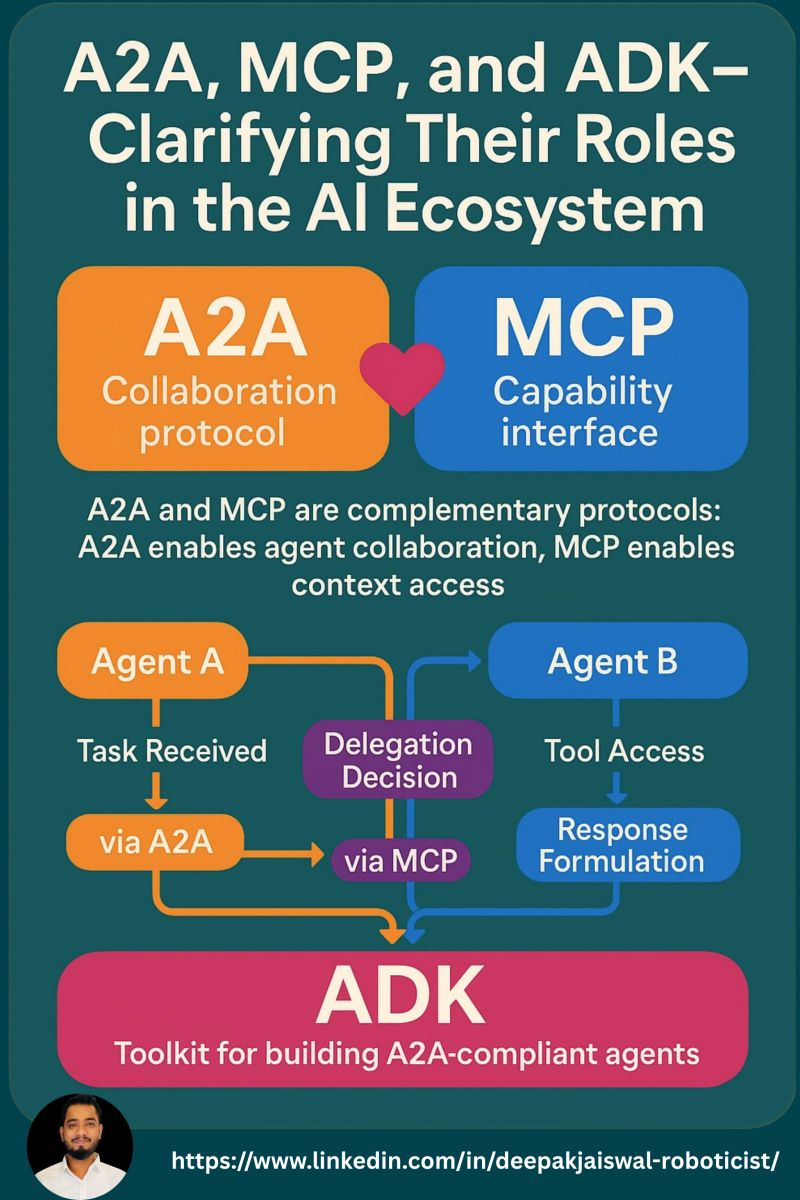
\includegraphics[width=0.4\linewidth,keepaspectratio]{agents7}
	\end{center}
	
{\tiny (Ref: LinkedIn post by Deepak Jaiswal)}

\end{frame}

%%%%%%%%%%%%%%%%%%%%%%%%%%%%%%%%%%%%%%%%%%%%%%%%%%%%%%%%%%%
\begin{frame}[fragile]\frametitle{Agentic AI Protocols Overview}
    \begin{itemize}
        \item A2A, MCP, and ADK are foundational for agentic systems.
        \item Each solves a unique challenge in building autonomous agents.
        \item They work together to enable scalable multi-agent architectures.
    \end{itemize}
\end{frame}

%%%%%%%%%%%%%%%%%%%%%%%%%%%%%%%%%%%%%%%%%%%%%%%%%%%%%%%%%%%
\begin{frame}[fragile]\frametitle{A2A: Agent-to-Agent Protocol}
    \begin{itemize}
        \item Enables agent discovery, delegation, and communication.
        \item Facilitates coordination in distributed multi-agent systems.
        \item Example: Agent A delegates a task to Agent B and receives results.
    \end{itemize}
\end{frame}

%%%%%%%%%%%%%%%%%%%%%%%%%%%%%%%%%%%%%%%%%%%%%%%%%%%%%%%%%%%
\begin{frame}[fragile]\frametitle{MCP: Model Context Protocol}
    \begin{itemize}
        \item Standardizes agent access to tools, APIs, and data.
        \item Ensures consistent, secure interaction with external systems.
        \item Example: Agent queries a database or triggers a payment via MCP.
    \end{itemize}
\end{frame}

%%%%%%%%%%%%%%%%%%%%%%%%%%%%%%%%%%%%%%%%%%%%%%%%%%%%%%%%%%%
\begin{frame}[fragile]\frametitle{ADK: Agent Development Kit}
    \begin{itemize}
        \item Toolkit for building A2A-compliant agents quickly.
        \item Includes libraries and scaffolds for rapid development.
        \item Compatible with frameworks like CrewAI, LangGraph, Semantic Kernel.
    \end{itemize}
\end{frame}

%%%%%%%%%%%%%%%%%%%%%%%%%%%%%%%%%%%%%%%%%%%%%%%%%%%%%%%%%%%
\begin{frame}[fragile]\frametitle{How They Work Together}
    \begin{itemize}
        \item \textbf{MCP}: Makes agents powerful with tool access.
        \item \textbf{A2A}: Enables inter-agent collaboration.
        \item \textbf{ADK}: Simplifies and accelerates agent development.
    \end{itemize}
\end{frame}

%%%%%%%%%%%%%%%%%%%%%%%%%%%%%%%%%%%%%%%%%%%%%%%%%%%%%%%%%%%
\begin{frame}[fragile]\frametitle{Real-World Analogy}
    \begin{itemize}
        \item \textbf{MCP}: Tools in a mechanic's toolbox.
        \item \textbf{A2A}: Team communication and task-sharing.
        \item \textbf{ADK}: Blueprint for building each mechanic fast.
    \end{itemize}
\end{frame}

%%%%%%%%%%%%%%%%%%%%%%%%%%%%%%%%%%%%%%%%%%%%%%%%%%%%%%%%%%%
\begin{frame}[fragile]\frametitle{Why This Stack Matters}
    \begin{itemize}
        \item Forms the backbone of enterprise AI, robotics, and automation.
        \item Enables modular, scalable, and intelligent agentic systems.
        \item Quickly becoming a standard for future AI workflows.
    \end{itemize}
\end{frame}


%%%%%%%%%%%%%%%%%%%%%%%%%%%%%%%%%%%%%%%%%%%%%%%%%%%%%%%%%%%%%%%%%%%%%%%%%%%%%%%%%%
\begin{frame}[fragile]\frametitle{}
\begin{center}
{\Large Anthropic :  How to Build AI Agents}

{\tiny (Ref; LinkedIn post by Maryam Miradi)}
\end{center}
\end{frame}

%%%%%%%%%%%%%%%%%%%%%%%%%%%%%%%%%%%%%%%%%%%%%%%%%%%%%%%%%%%
\begin{frame}[fragile]\frametitle{When to Build AI Agents}
    \begin{itemize}
        \item Don’t build agents for every task.
        \item Ideal for complex, ambiguous, high-value problems.
        \item Use workflows when decision paths are clear.
        \item Agents consume tokens—ensure value justifies cost.
        \item Avoid if error discovery is slow or high-risk.
        \item Limit autonomy when safety is critical.
        \item Use checklist: complexity, value, bottlenecks, risks.
        \item Coding is a great fit: complex but verifiable.
    \end{itemize}
\end{frame}

%%%%%%%%%%%%%%%%%%%%%%%%%%%%%%%%%%%%%%%%%%%%%%%%%%%%%%%%%%%
\begin{frame}[fragile]\frametitle{Designing Simple, Scalable Agents}
    \begin{itemize}
        \item Every agent = Model + Tools + Environment.
        \item Start with extremely simple components.
        \item Avoid early complexity—hurts iteration speed.
        \item Reuse agent backbones for many use cases.
        \item Recombine code, tools, and prompts easily.
        \item Don’t optimize until behavior is stable.
        \item Visual clarity builds trust in the agent.
    \end{itemize}
\end{frame}

%%%%%%%%%%%%%%%%%%%%%%%%%%%%%%%%%%%%%%%%%%%%%%%%%%%%%%%%%%%
\begin{frame}[fragile]\frametitle{Optimization \& Performance}
    \begin{itemize}
        \item Parallelize tools to lower latency.
        \item Cache action paths in coding agents to save tokens.
        \item Show step-by-step progress to build trust.
        \item Optimize costs only after validating core loop.
        \item Keep environments simple before scaling up.
    \end{itemize}
\end{frame}

%%%%%%%%%%%%%%%%%%%%%%%%%%%%%%%%%%%%%%%%%%%%%%%%%%%%%%%%%%%
\begin{frame}[fragile]\frametitle{Think Like Your Agent}
    \begin{itemize}
        \item Agent only sees its limited context window.
        \item Don’t expect magic—expect bounded reasoning.
        \item Weird actions often mean missing context.
        \item Simulate tasks from the agent’s view.
        \item Debug using only the agent’s available info.
        \item Poor UI? Add metadata or improve resolution.
        \item Replay full trajectory—ask the model “why?”
    \end{itemize}
\end{frame}

%%%%%%%%%%%%%%%%%%%%%%%%%%%%%%%%%%%%%%%%%%%%%%%%%%%%%%%%%%%
\begin{frame}[fragile]\frametitle{Tools \& Self-Improvement}
    \begin{itemize}
        \item Define tools with clear inputs and expected outputs.
        \item Use the LLM to review tool clarity.
        \item Let agents self-critique prompts and tools.
        \item Build meta-tools that improve agent tooling.
        \item Better ergonomics reduce errors and retries.
    \end{itemize}
\end{frame}

%%%%%%%%%%%%%%%%%%%%%%%%%%%%%%%%%%%%%%%%%%%%%%%%%%%%%%%%%%%
\begin{frame}[fragile]\frametitle{The Future: Multi-Agent \& Budget-Aware}
    \begin{itemize}
        \item Solo agents dominate now—but not for long.
        \item Multi-agent = modular reasoning + parallel tasks.
        \item Sub-agents help preserve main context window.
        \item Async interactions beat synchronous limitations.
        \item Role-based coordination is the next big step.
        \item Budget-awareness = tokens, time, latency constraints.
        \item Define strict resource limits before deployment.
    \end{itemize}
\end{frame}

